\documentclass{beamer}
\usepackage[utf8]{inputenc}
\usepackage[spanish,es-tabla]{babel}
\usepackage{graphicx}
\graphicspath{ {imagenes/} }

\usetheme{PaloAlto}

\title{Paralelización de RSA con Open MPI y POSIX Threads}

\author{Christofer Chávez Carazas}


\institute[Universidad Nacional de San Agustín] 


\date{\today}

\subject{Proyectos I}
\AtBeginSubsection[]
{
  \begin{frame}<beamer>{Outline}
    \tableofcontents[currentsection,currentsubsection]
  \end{frame}
}

\begin{document}

\begin{frame}
  \titlepage
\end{frame}

\begin{frame}{Motivación}
  \begin{itemize}
   \item Operaciones con números grandes.
   \item Paralelizar la exponenciación modular con \textit{OpenMP} para reducir el tiempo de encriptado y desencriptado.
   del \textit{RSA}
   \item Creación de hilos inecesarios.
  \end{itemize}
\end{frame}


\begin{frame}{RSA}
 \begin{itemize}
  \item Sistema criptográfico asimétrico.
  \item Seguridad basada en dos números primos grandes.
  \item Usa al exponenciación modular.
 \end{itemize}
\end{frame}

\begin{frame}{Generación de llaves}
  \begin{enumerate}
   \item Se escogen aleatoriamente dos números primos grandes \textit{q} y \textit{p}.
   \item Se obtiene el módulo $n = q * p$.
   \item Se calcula  $\varphi(n) = (p-1)(q-1)$
   \item Se selecciona un \textit{e} que cumpla: $1 < e < \varphi(n)$ y que sea coprimo con $\varphi(n)$.
   \item Se selecciona un \textit{d} que cumpla: $1 < d < \varphi(n)$ tal que $e*d = 1\:mod\:\varphi(n)$.
  \end{enumerate}
\end{frame}

\begin{frame}{Cifrado y Descifrado}
  \begin{block}{Cifrado}
    $$c \equiv m^{e} (mod\:n)$$ 
    Donde \textit{c} es el mensaje cifrado, \textit{m} es el mensaje original, \textit{e} es la llave pública y
    \textit{n} es el módulo hallado anteriormente.
  \end{block}
  \begin{block}{Descifrado}
   $$m \equiv c^{d} (mod\:n)$$
   Donde \textit{m} es el mensaje original, \textit{c} es el mensaje cifrado, \textit{d} es la llave privada y
   \textit{n} es el módulo hallado anteriormente.
  \end{block}
\end{frame}

\begin{frame}{Repeated square-and-multiply Algorithm}
  El algoritmo se basa en la siguiente observación:
  $$g^{e} mod\:m = (g^{e/2} * g^{e/2}) mod\:m$$
  y se puede definir recursivamente de la siguiente manera:
  \begin{figure}
   \centering
   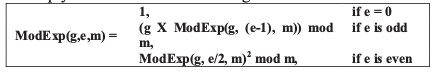
\includegraphics[scale = 0.5]{1.png}
   \caption{\textit{Repeated square-and-multiply} \cite{Paper}}
   \label{fig:1}
  \end{figure}
\end{frame}

\begin{frame}{Exponenciación Modular binaria Paralela}
\begin{itemize}
 \item Se convierte el exponente a su forma binaria y se lo divide en k partes dependiendo del número de procesadores.
 \item La exponenciación tendría la siguiente forma:
 $$g^{e} = g^{2^{r_{k}}e_{k}} \cdots g^{2^{r_{2}}e_{2}}*g^{2^{r_{1}}e_{1}}$$
 siendo las \textit{r} calculadas de la siguiente forma:
 $$r_{1} = 0, r_{2} = \frac{n}{k}, r_{3} = \frac{2n}{k},\cdots,r_{k} = \frac{(k-1)n}{k}$$
 \item Cada parte se calcula con el \textit{Repeated square-and-multiply Algorithm}
\end{itemize}
\end{frame}

\begin{frame}{Propuesta}
  \begin{itemize}
   \item Utilizar \textit{Open MPI} para paralelizar el cifrado y descifrado del mensaje.
   \item Utilizar \textit{POXIS Threads} para paralelizar la exponenciación modular.
   \item Optimizar la creación de hilos y la distribución de los datos.
  \end{itemize}
\end{frame}


\begin{frame}{Distribución en MPI}
  \begin{itemize}
   \item Se distribuye el mensaje entre los procesos.
   \item Se convierte la key en su forma binaria y se copia en todos los procesos.
  \end{itemize}
\end{frame}

\begin{frame}{Distribución en Pthreads}
  \begin{itemize}
   \item Se crea una matriz compartida entre los hilos.
   \item Cada hilo opera una columna de la matriz.
   \item Se crea un array compartido entre los hilos.
   \item Se reparten las filas de la matriz entre los hilos.
   \item El resultado de la multiplicación se guarda en el array.
  \end{itemize}
\end{frame}


\begin{frame}
 \begin{figure}
  \centering
  
\includegraphics[scale = 0.6]{4.png}
 \end{figure}
\end{frame}

\begin{frame}{SetUp}
 Los experimentos se realizaron en el supercomputador de la UNSA
 \begin{itemize}
  \item GPUs: 24 x 2.60 GHz.
  \item Memory(RAM): 62.90 GB.
  \item SO: Linux 3.10.0-514.16.1.el7.x86 64 (x86 64).
 \end{itemize}
\end{frame}

\begin{frame}{Características de los experimentos}
  \begin{itemize}
   \item Llaves de 512 bits y 1024 bits.
   \item Combinaciones entre el número de nodos (1,2,4,6) y el número
    de hilos por nodo (1,2,4,8,16,24).
    \item Tres mensajes generados aleatoriamente de tamaños 1024, 4096, 16392 caracteres.
   \item Cada experimento se ejecutó 25 veces y se sacó el promedio.
  \end{itemize} 
\end{frame}



\begin{frame}{Resultados con key de 512 bits}
 \begin{figure}
  \centering
  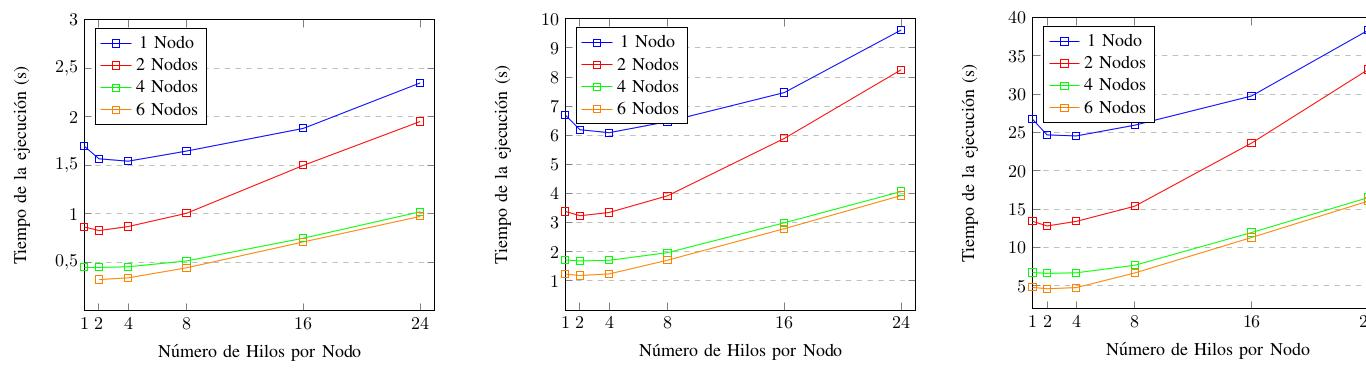
\includegraphics[scale = 0.28]{5.jpeg}
 \end{figure}
\end{frame}

\begin{frame}{Resultados con key de 1024 bits}
 \begin{figure}
  \centering
  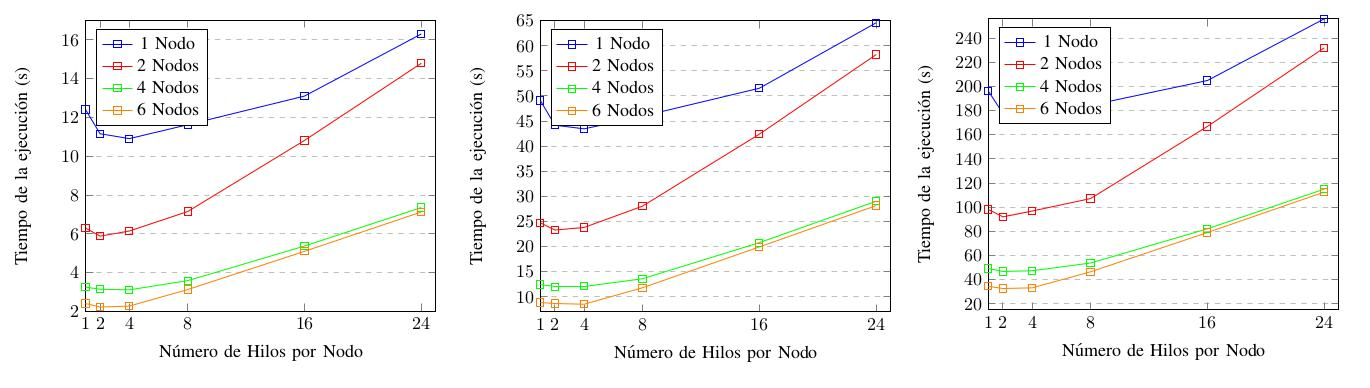
\includegraphics[scale = 0.28]{6.jpeg}
 \end{figure}
\end{frame}


\begin{frame}{Conclusiones}
 \begin{itemize}
  \item Se logra paralelizar el RSA de forma optima en la parte de MPI.
  \item Aunque se pueda ganar tiempo al no crear más hilos de los necesarios, se necesita de más memoria para guardar las matrices creadas en cada proceso.
 \end{itemize}
\end{frame}



\begin{frame}
\begin{thebibliography}{}
\setbeamertemplate{bibliography item}[article]
\bibitem[S. Saxena et al. 2014]{Paper} Sapna Saxena, Bhanu Kapoor \textbf{An Efficient Parallel Algorithm for Secured Data Communications Using RSA Public Key Cryptography Method}, 2014.
\end{thebibliography}
\end{frame}

\end{document}


